\documentclass[10pt]{llncs}
\usepackage[utf8]{inputenc}
\usepackage{graphicx}

\begin{document}
\title{Blockchain applications to secure data transfer systems creation}
\author{Gleb Slepenkov\inst{1}\orcidID{0009-0001-9978-396X}}
\authorrunning{G. Slepenkov}
\institute{Saint Petersburg State University, 7-9 Universitetskaya Embankment, St Petersburg, Russia, 199034}

\maketitle

\section{Introduction}

In contemporary information societies, secure data transmission (SDT) is paramount for maintaining data confidentiality and integrity. 
SDT systems are critical infrastructure components across diverse sectors, including financial institutions, governmental agencies, and enterprise.

Implementing robust SDT mechanisms becomes particularly challenging when facilitating cross-organizational data exchange or connecting geographically dispersed departments within a single organization. 
Such scenarios necessitate data transfer across external, public networks, thereby significantly elevating the risk of unauthorized data disclosure or modification during transit. 
Consequently, rigorous data integrity verification and sender authentication protocols are indispensable. 
Furthermore, confirmation of data reception is often a critical requirement. 
The heterogeneity of data exchange technologies employed by different entities can further complicate the SDT process.

Blockchain represents an emerging technology for SDT solutions. 
This technology by design provides core features essential for SDT such as fault tolerance, ledger data immutability, zero trust between blockchain nodes.
Moreover, many blockchains are designed to operate in unreliable public networks with nodes running in different heterogeneous clusters owned by separate stakeholders.
By this reason blockchains are especially suitable for cross-organizational data transfer.
Furthermore, blockchain platforms often provide smart contracts which allow to implement custom data transfer logic directly on blockchain.  

This study investigates existing paradigms of blockchain applications to SDT process and proposes a new approach, which allows to combine advantages of existing paradigms and create 
SDT blockchain-based system, which preserves key features of existing approaches, but has message broker like architecture and lax data size limitations.
The study is organized in a following way. 
In section \ref{related_work} existing data transfer paradigms are described in detail.
In section \ref{architecture} proposed system architecture is presented.
In section \ref{implementation_details} implementation details of created systems are described.
In section \ref{further_research_directions} further research directions are provided.

\section{Related Work} \label{related_work}

The integration of blockchain technology into data transfer systems presents two primary paradigms: blockchain as a data access interface and blockchain as a direct data transfer tool. 
This section examines the existing literature, classifying studies according to these two distinct roles of blockchain in facilitating data exchange.

\subsection{Blockchain as a Data Access Interface}

This approach leverages blockchain as a secure and transparent mechanism for managing and controlling access to data that is typically stored off-chain. 
The blockchain records metadata about the data, access permissions, and transaction histories, thereby ensuring data integrity, auditability, and secure access control.
The data itself is transferred using conventional methods.

\cite{Wang2024} introduced BBS, a big data sharing system utilizing blockchain for access control and data integrity management. 
Similarly, \cite{WangYY2021} proposed a blockchain-based model for sharing big data in the oil and gas sector, employing blockchain to enable secure data access and provenance tracking. 
\cite{Yang2022} developed a sharing platform for wild bird data based on blockchain and IPFS, where blockchain governs access rights to data residing in IPFS. 
\cite{Jia2023} presented a cross-organizational data sharing framework that uses blockchain probes to orchestrate and audit data access across various entities. 
\cite{Gupta2022} explores the application of blockchain for securing data access within e-healthcare applications.

\subsection{Blockchain as a Data Transfer tool}

This approach employs the blockchain directly to transfer data between participants. While data may occasionally be stored on-chain, it is more common for the blockchain to facilitate the transfer of data stored off-chain, often in conjunction with technologies such as peer-to-peer networks or distributed file systems.

\cite{Lin2023} proposed a multi-level blockchain architecture for secure data transfer in the Internet of Vehicles (IoV), directly leveraging blockchain for data exchange. \cite{Peng2023} demonstrated the feasibility of building a peer-to-peer file storage and sharing system on a consortium blockchain, where the blockchain assists in discovering and securely transferring file chunks. \cite{Priyadarshini2021} introduced a system for secured data transfer between fog nodes utilizing blockchain to enhance the security of the data transfer process itself.

\subsection{Enabling Technologies and Security Considerations}

Regardless of the chosen paradigm, several enabling technologies and security considerations are universally relevant.
\cite{kim2020hybrid} presented a hybrid decentralized PBFT blockchain framework for OpenStack message queues, aimed at improving fault tolerance and scalability, 
crucial aspects for reliable data transfer systems. 
\cite{Ghaemi2021} introduced a publish-subscribe architecture to foster interoperability among different blockchain networks, thus facilitating data exchange across heterogeneous systems. 
\cite{Bagga2021} and \cite{Xu2021} explored blockchain-based authentication and key agreement protocols for IoV, enhancing the security of data transfer in vehicular contexts. 
\cite{Bogdanov2024} focused on the consensus mechanism, exploring a combination of PBFT and Raft, while \cite{Ai2022} proposed a Proof-of-Transactions consensus protocol, 
both striving for efficient and scalable agreement in distributed ledgers. \cite{Lin2020} focused on developing a privacy-preserving authentication protocol specifically for VANETs. 
\cite{Bagga2022} surveyed blockchain applications in smart transport, including those involving data transfer. 
\cite{Song2023} provides a comprehensive survey of blockchain-based data sharing schemes, encompassing both categories detailed in this section.

\subsection{Comparison of Approaches}

The two approaches, blockchain as a data access interface and blockchain as a data transfer tool, offer distinct advantages and disadvantages depending on the specific use case and requirements.

\begin{table}[h!]
\caption{Comparison of Blockchain Approaches for Data Transfer}
\label{tab:comparison}
\begin{tabular}{|p{20mm}|p{50mm}|p{50mm}|}
\hline
Feature & Blockchain as Data Access Interface & Blockchain as Data Transfer tool \\ \hline
Data Storage & Primarily Off-Chain & Often Off-Chain, but metadata on-chain \\ \hline
Data Transfer & Traditional methods & Blockchain or Blockchain-assisted \\ \hline
Scalability & Higher, as data transfer is off-chain & Potentially Lower, dependent on blockchain throughput \\ \hline
Complexity & Lower & Higher \\ \hline
On-Chain Footprint & Smaller (Metadata only) & Larger (Metadata and potentially data chunks) \\ \hline
Suitability & Large datasets, access control focus & Smaller datasets, secure and direct transfer focus \\ \hline
\end{tabular}

\end{table}

As illustrated in Table \ref{tab:comparison}, the choice between these two approaches hinges on factors such as data size, scalability requirements, security priorities, 
and the level of on-chain transparency desired. 
The data access interface approach is generally more suitable for scenarios involving large datasets and a primary focus on secure access control, while the data transfer tool 
approach is better suited for scenarios demanding secure and direct data transfer, even if it potentially introduces limitations in terms of scalability.

\section{Proposed system architecture} \label{architecture}

This section describes the architecture of proposed system.
The main goal of such an architecture is to make a combination of two main blockchain integration into data transfer systems described in section \ref{related_work}
in order to create system with message broker like architecture, convenient for data transfer, and lax data size limitations comparing to existing solutions.
Essentially architecture follows the trends described in related articles:

\begin{enumerate}
    \item Blockchain usage as message broker: \cite{kim2020hybrid}, \cite{Ghaemi2021}. 
    The key drawback of theese solutions lies in usage of ledger for message transfer.
    It greatly limits the system scalability and transfered data size. 
    \item Blockchain as interface to off-chain data (e.g. \cite{Wang2024}, \cite{Jia2023}).
    Such a solutions usually do not have any notification mechanisms.
    Hence, message receiving becomes a challenging task.
\end{enumerate}

Proposed architecture assumes that system should contain the following components:

\begin{itemize}
    \item Blockchain as main data transfer tool. 
    \item Data storages internaly used by counterparties (organizations) to store the data to be sent;
    \item Connectors --- some application used by SDT process counterparties in order to create connection between their data storages
    and blockchain nodes owned by organization (mainly inspired by blockchain probes described in \cite{Jia2023})
\end{itemize}

A sample of such an architecture for SDT between two organizations is presented on figure \ref{system_architecture}.

\begin{figure}
    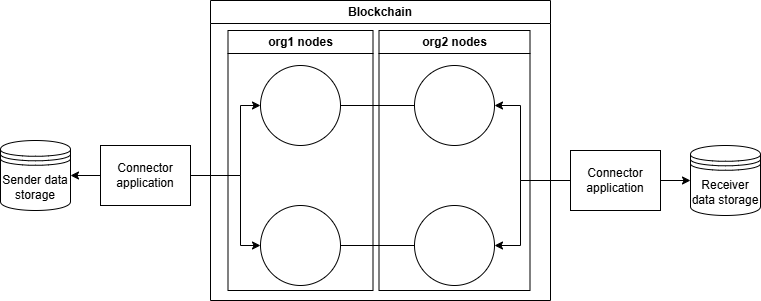
\includegraphics[width=\textwidth]{system_architecture.png}
    \caption{System architecture for two organizations} \label{system_architecture}
\end{figure}

The SDT process is presented on figure \ref{sending_process}.
It represents the following algorighm:

\begin{enumerate}
    \item Data sender (org1) initiates process by sending data transfer request to connector it uses to integrate with blockchain.
    \item Org1 connector stores the data into org1 storage and collects metadata for data transfered.
    \item Org2 connector sends request to blockchain and initiates SDT smart contract execution.
    \item Smart contract validates metadata and stores it into ledger.
    \item Smart contract notifies message receiver (connector of org2) about new message existence.
    \item Smart contract confirms message delivery acceptance to org1.
    \item Org2 connector requests data from blockchain by sending request to org2 blockchain nodes and executing SDT smart contract.
    \item Smart contract validates org2 permissions on requested data.
    \item Smart contract request data from org1 connector.
    \item Org1 connector receives data from org1 storage and returns it to smart contract.
    \item Smart contract prepares data for transfer.
    On this stage data could be encrypted and signed according to smart contract implementation.
    \item Smart contract returns prepared data to org2 connector.
    \item Org2 connector stores data into org2 storage.
    \item Org2 connector notify blockchain about message receiving by using smart contract.
    \item Smart contract marks message in registry as delivered.
    \item Smart contract notifies org1 connector about message delivery process completion.
    \item Org1 connectors notifies data sender about message delivery process completion. 
\end{enumerate}

\begin{figure}
    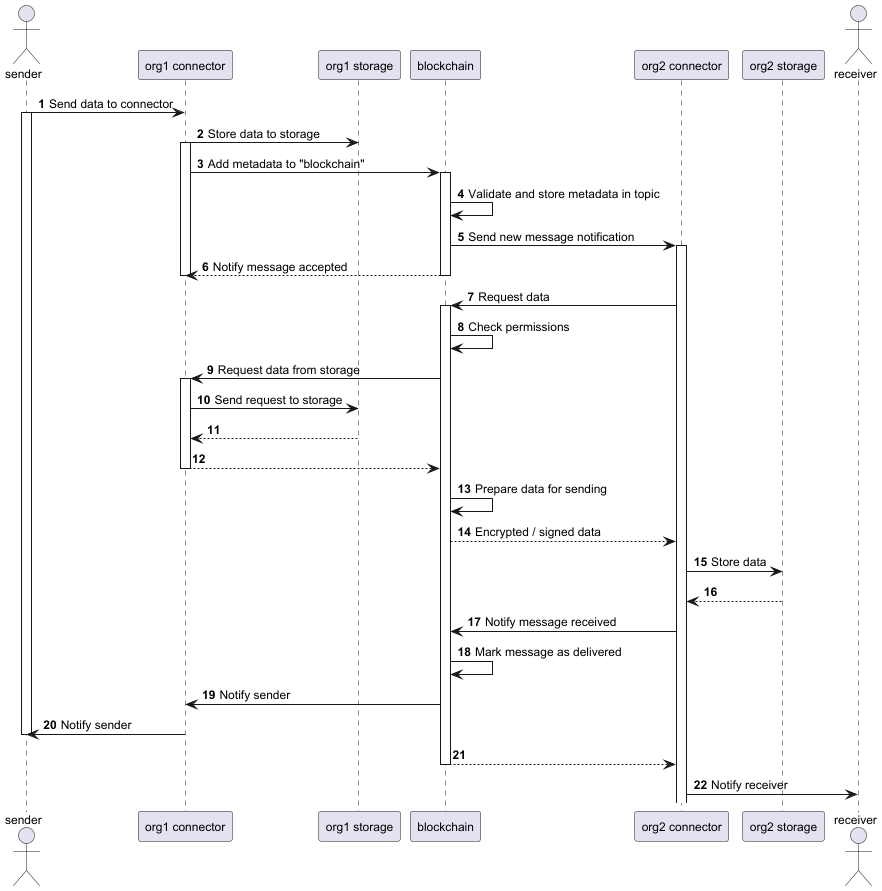
\includegraphics[width=\textwidth]{sending_process.png}
    \caption{SDT process scheme} \label{sending_process}
\end{figure}

Such an algorighm has following important features:

\begin{enumerate}
    \item Loose coupling between sender and receiver due to blockchain usage as message broker.
    \item Better fault tolerance comparing to regular message brokers.
    \item More convenient message broker like SDT interface comparing to existing blockchain solutions.
    \item Great SDT process customization capabilities due to smart contract usage.
\end{enumerate}


\section{Implementation details} \label{implementation_details}

\section{Further research directions} \label{further_research_directions}

\bibliographystyle{splncs04}
\bibliography{references}

\end{document}